% !TEX root=/home/tavant/these/manuscript/src/manuscript.tex

\section{Monte Carlo computation of the EVDF}
\label{sec-MCM}
  
  The \ac{1D} \ac{PIC} simulations were computed faster than the \ac{2D} simulations, as the latter needed around a week to compute $10\,\micro\second$ on 360 CPUs, while the former needed only a few days on 64 CPUs to compute $20\,\micro\second$ of physical time.
  However, they still took a rather long time, especially when compared to fluid models that can be solve from under one second to around one day on a single core, depending of the hypotheses used.
  
  We have seen that the the polytropic index depends on several conditions, as the background pressure (see \cref{fig-p}) but also the densities, sizes, heating mechanism, and so on.
  We have seen in \cref{sec-fluid} that the only value of the polytropic index $\gamma$ is enough to describe the \ac{PIC} simulation.
  As the value of $\gamma$ depends on the \ac{EVDF}, we propose here a Monte Carlo approach that could be used in order to obtain the \ac{EVDF} faster that a \ac{PIC} simulation.
  A possible application would be similar to \citet{kushner1983}, where the author uses a small population of electrons (typically 300-500) and observes their evolutions in a given plasma potential.
  
  This method gets rid of the Poisson equation, which can take between 30\% and 50\% of the total simulation time.
  Hence, the Debye length does not have to be highly resolved any more for stability and numerical heating.
  However, we still need to resolve the sheath, which length is of the order of 5 Debye lengths \citep{chabert2014}.
  Consequently, a coarser mesh of cell size 5 times larger can be used.
  The condition on the time step is also reduced.
  This results in a much faster computation.

  \subsection{Description of the Monte Carlo approach}

    In order to validate the Monte Carlo approach, we use the converged simulation of the \ac{1D} \ac{PIC} model.
    We uses the potential, so the electric field, computed self-consistently in the \ac{PIC} simulation.
    The Monte Carlo is initialised with a uniform density of electrons.
    When an electron is collected at the wall, it is re-injected, similarly to the \ac{PIC} simulation.
    The electrons are pushed, and undergo collisions as described in \cref{sec-elements}.

    We validate the Monte Carlo computation by comparing the electron density, temperature and distribution function.
    \Cref{fig-EEPF_start_end} shows the expected EEPF obtained in the \ac{PIC} simulation with a background pressure of $P=1$\,mTorr.
    The maximum plasma potential, at the center of the domain, is $\max(\phi)=12.2\,\volt$.
    Is also shown in \cref{fig-EEPF_start_end} the EEPF at the beginning of the Monte Carlo computation, which corresponds to the Maxwellian distribution of temperature $\Te=5\,\volt$

    \begin{figure}[hbtp]
      \centering
      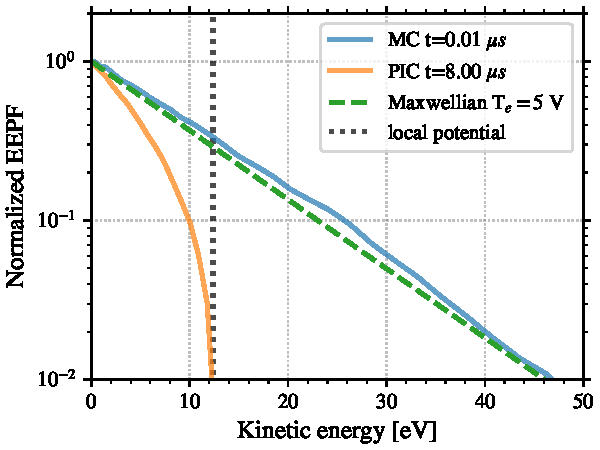
\includegraphics[width=\defaultwidth]{EEPF_PIC}
      \caption{Electron energy probability function obtained from (orange) the PIC simulation after convergence, and (blue) at the beginning of the Monte Carlo simulation. Is overlaid the local plasma potential.}
      \label{fig-EEPF_start_end}
    \end{figure}
    \improvement{\cref{fig-EEPF_start_end}: Maxwellian + $\Te$ in V, not eV}

    \paragraph{Time scales \\}
    The electrons collected at the wall have a kinetic energy at least equal to the potential drop to the wall $\ek = e \dphi$, which corresponds in our case to a limit velocity of $v_{\rm lim} = \sn{1.5}{6} \,\meter\per\second$.
    Hence, the limit time of flight between the two boundaries is
    \[ T_{\rm flight} = \frac{L}{v_{\rm lim}} = 0.068 \,\micro\second  \]

    \vspace{1em}
    The electron-neutral scattering frequency is computed for a background pressure of $0.13$\,bar (${100}$\,mTorr) at the temperature of $300\,\kelvin$, which corresponds to a neutral density of $${n_g = \sn{3.2}{21} \meter^{-3}}.$$
    For an electron temperature of $5\,\volt$, the thermal electron-neutral elastic scattering frequency is 
    \[ \nu_{\rm ela} = 205 \,\mega\hertz.  \] 

    However, at this high energy, electron-neutral scattering is not isotropic, but instead gives mostly small angles (forward scattering) \citep{vahedi1995}.
    Hence, a large number of collision is required.
    The resulting time scale corresponding of the electron-neutral scattering is of the order of 
    \[ T_{\rm ela} \simeq \frac{100}{\nu_{\rm ela}} = 0.4 \,\micro\second  \]
    
    \inlinenote{Here, 1/$\nu = 0.004$, I don"t know why it is that low, while the MC calculations takes much more time to thermalize... Maybe due to the Injection ? \\ Anne: En regardant les temps sur tes resultats apres, j'ai compris ce qui te posait probleme ici. Tu es sur que dans ton monte carlo, ta densité de neutres n'est pas trop faible?}

    \paragraph{Numerical artefacts \\}
    In PIC simulations, numerical parameters can induce numerical heating and thermalization \citep{lai2014}.
    The numerical heating has been studied in detail \citep{birdsall1991}.
    It is due to aliasing effects, and depends of the grid size, time step and number of particles per cell.
    The choice of these parameter leads to reduce the effect of the heating.

    The thermalization is the fact that the distribution of the particle tends toward a Maxwellian.
    It originates from fluctuations of the electric field due to the discretization of the particle.
    The first studies showed that the thermalization time $\tau_T$ depends on $N_D$ the number of (numerical) particles per Debye sphere \citep{dawson1964,montgomery1970}.
    The presence of collisions can affect $\tau_T$  \citep{turner2006,lai2014}.
    In \citet{turner2006}, the author observed the evolution of the thermalization time with $N_D$ as
    \begin{equation} \label{eq-taut}
      \tau_T = \frac{1}{\omega_{pe}} \frac{34.4}{N_D^{-2} + 28.0 N_D^{-1} \frac{\nu_m}{\omega_{pe}}}
    \end{equation}
    which gives in our condition a time-scale several orders of magnitude larger than the other time scales $T_{\rm ela}$ and $T_{\rm flight}$ .
    Hence, the effects of numerical parameters on the kinetics informations of the simulation are expected to be negligible.


  \subsection{Results of the Monte Carlo computation} \label{subsec-MCMresults}

    We measured the electron energy distribution function (EEDF) at $3\,\centi\meter$ from the left wall.
    \Cref{fig-zoom_init_Mc} shows the evolution of the EEDF at the very early moments of the simulation, from $t=0.01$ to $0.08\,\micro\second$.
    The energy of the electrons is oriented, meaning that the electrons with positive energy are coming from the wall, while the negative energy is used for the electrons going toward the wall.

    \begin{figure}[hbtp]
      \centering
      \begin{tabular}{cc}
        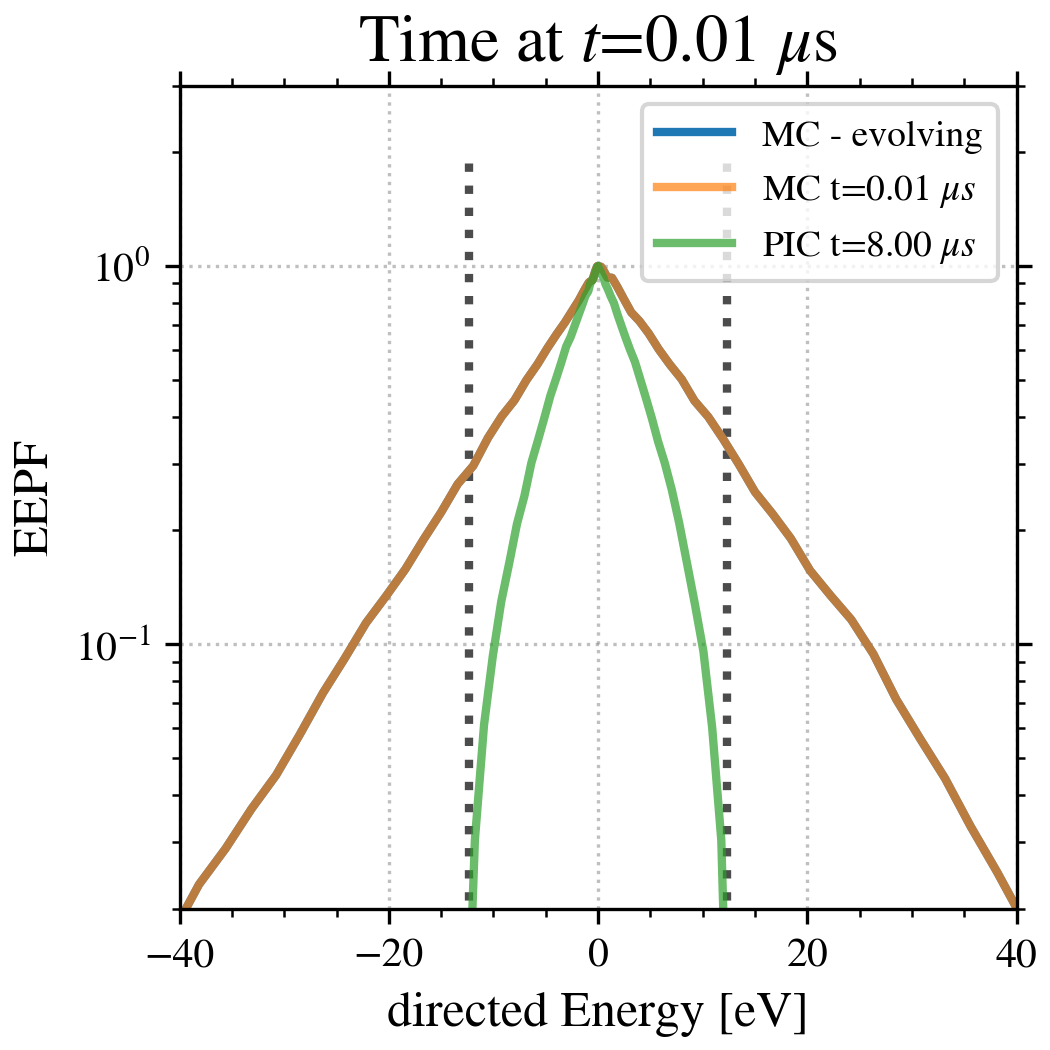
\includegraphics[width=0.4\textwidth]{MCC_EEDF/Heelo_1} &
        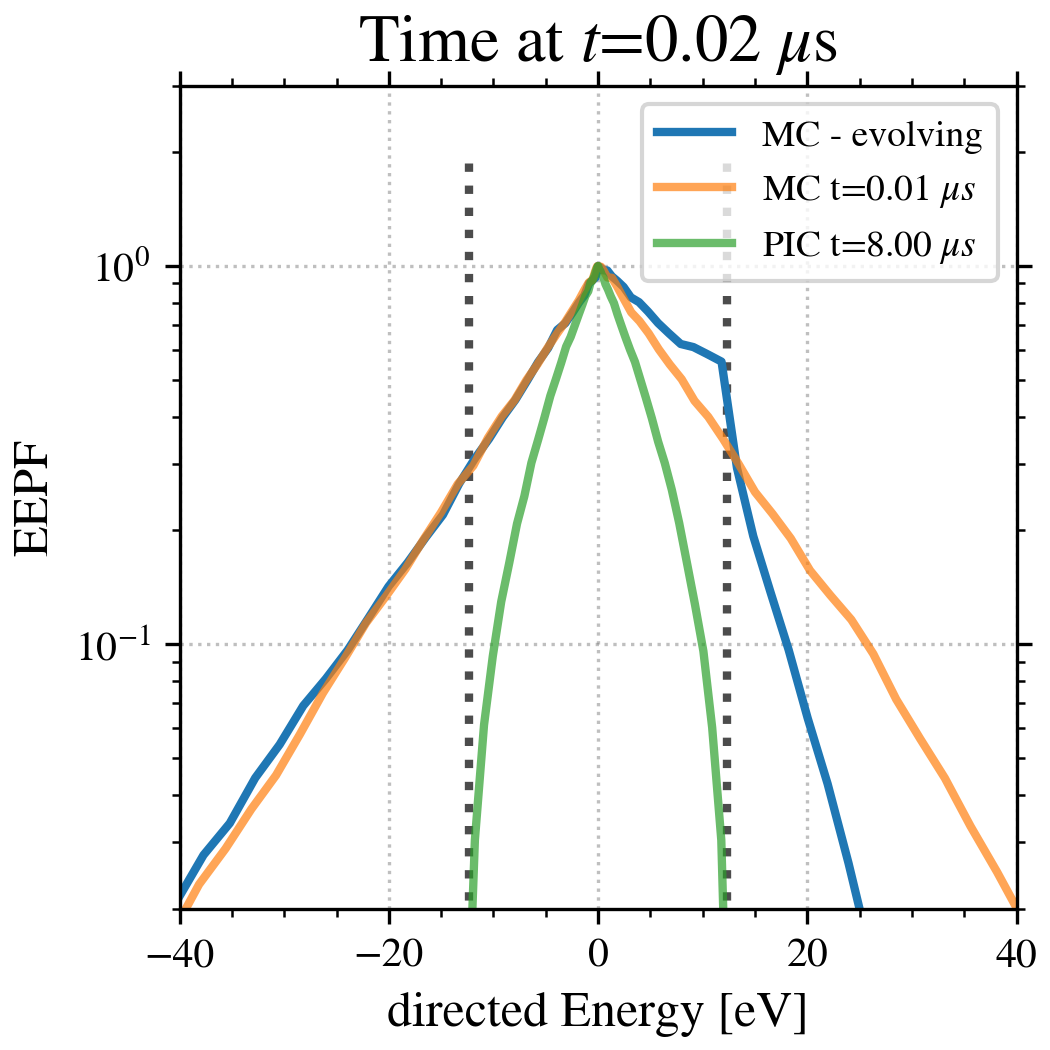
\includegraphics[width=0.4\textwidth]{MCC_EEDF/Heelo_2} \\
        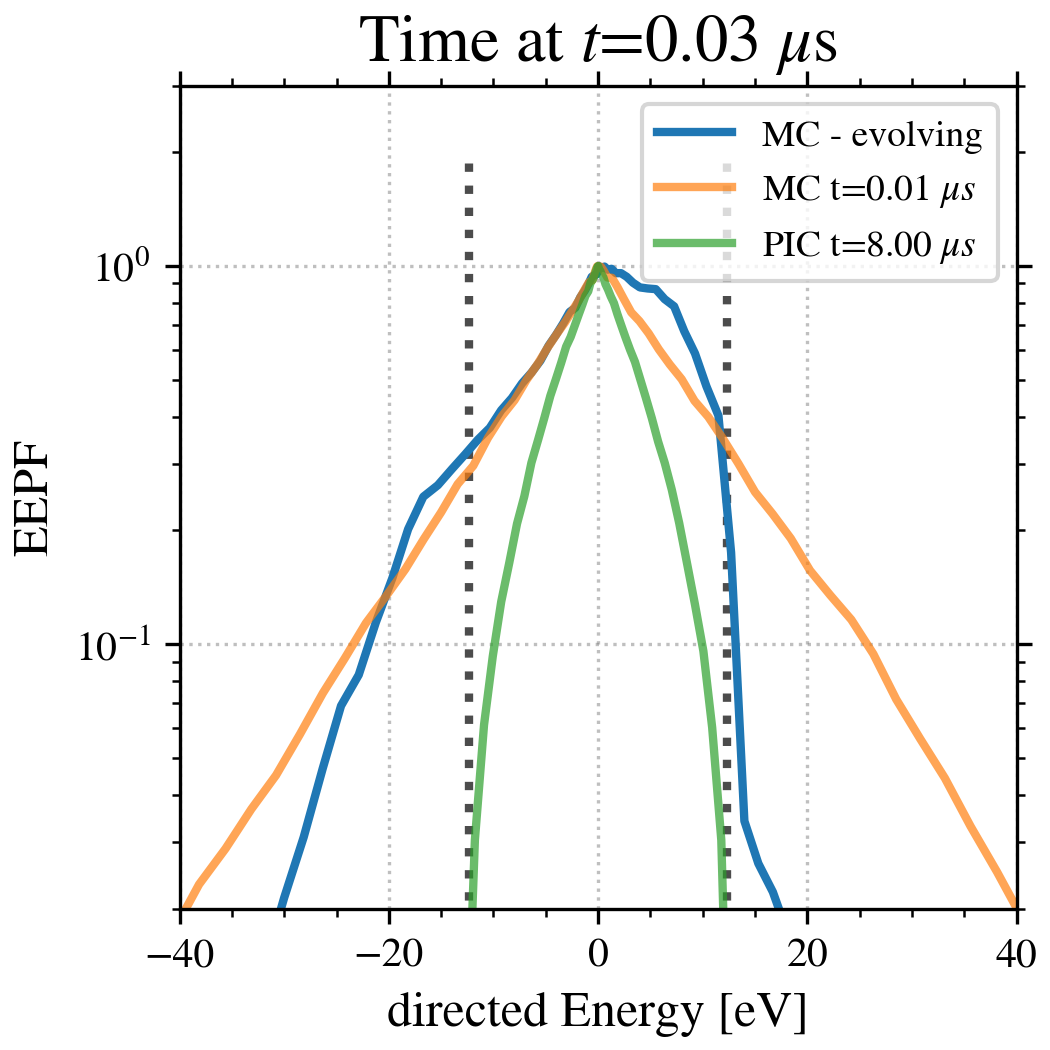
\includegraphics[width=0.4\textwidth]{MCC_EEDF/Heelo_3} &
        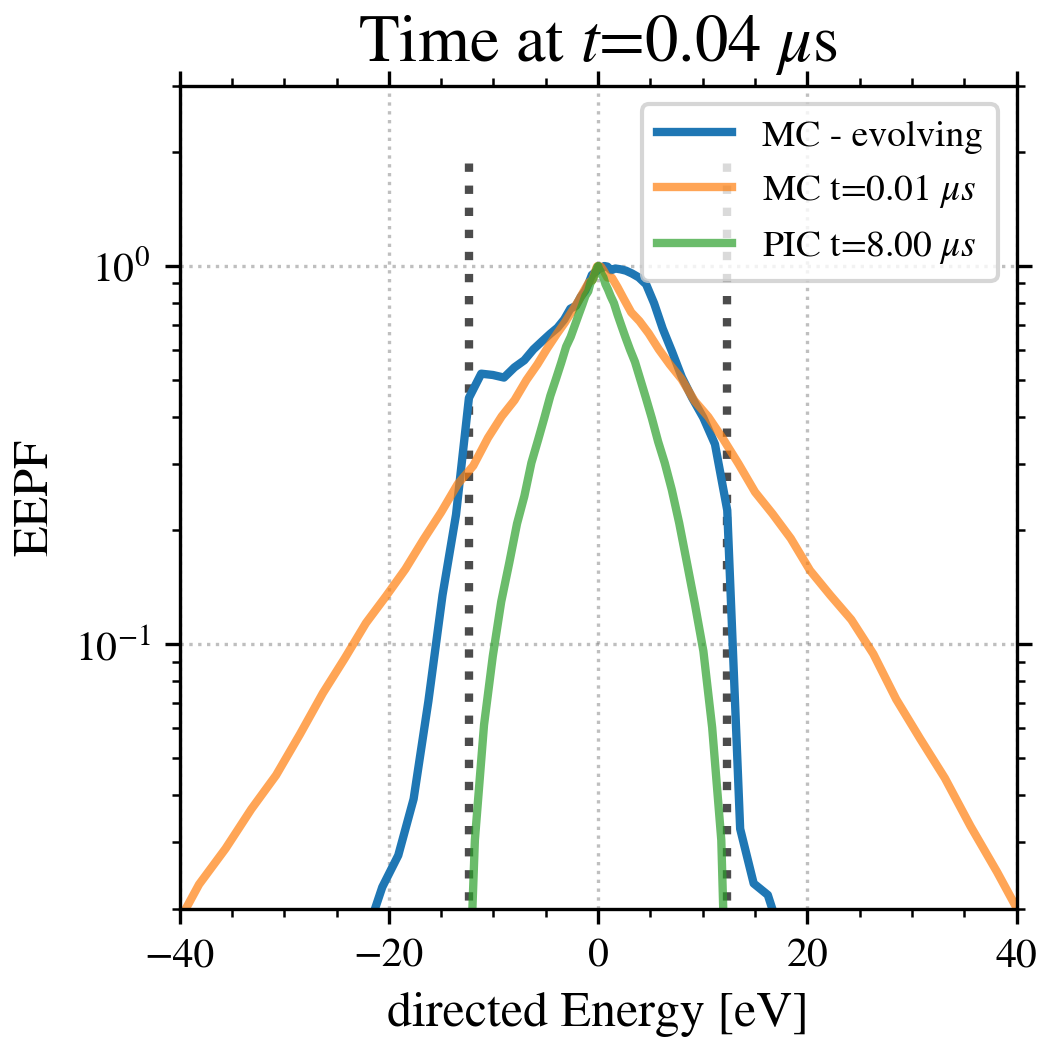
\includegraphics[width=0.4\textwidth]{MCC_EEDF/Heelo_4} \\
        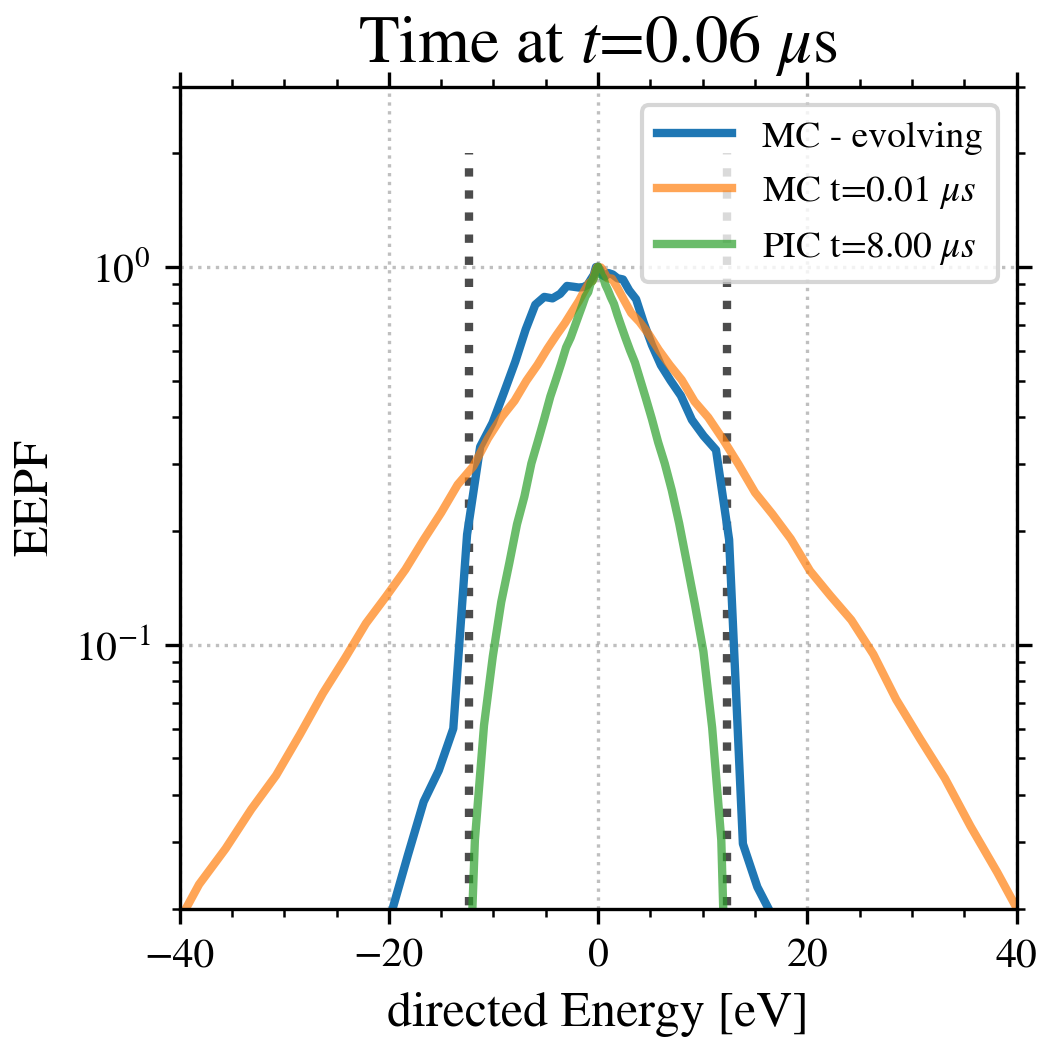
\includegraphics[width=0.4\textwidth]{MCC_EEDF/Heelo_6} &
        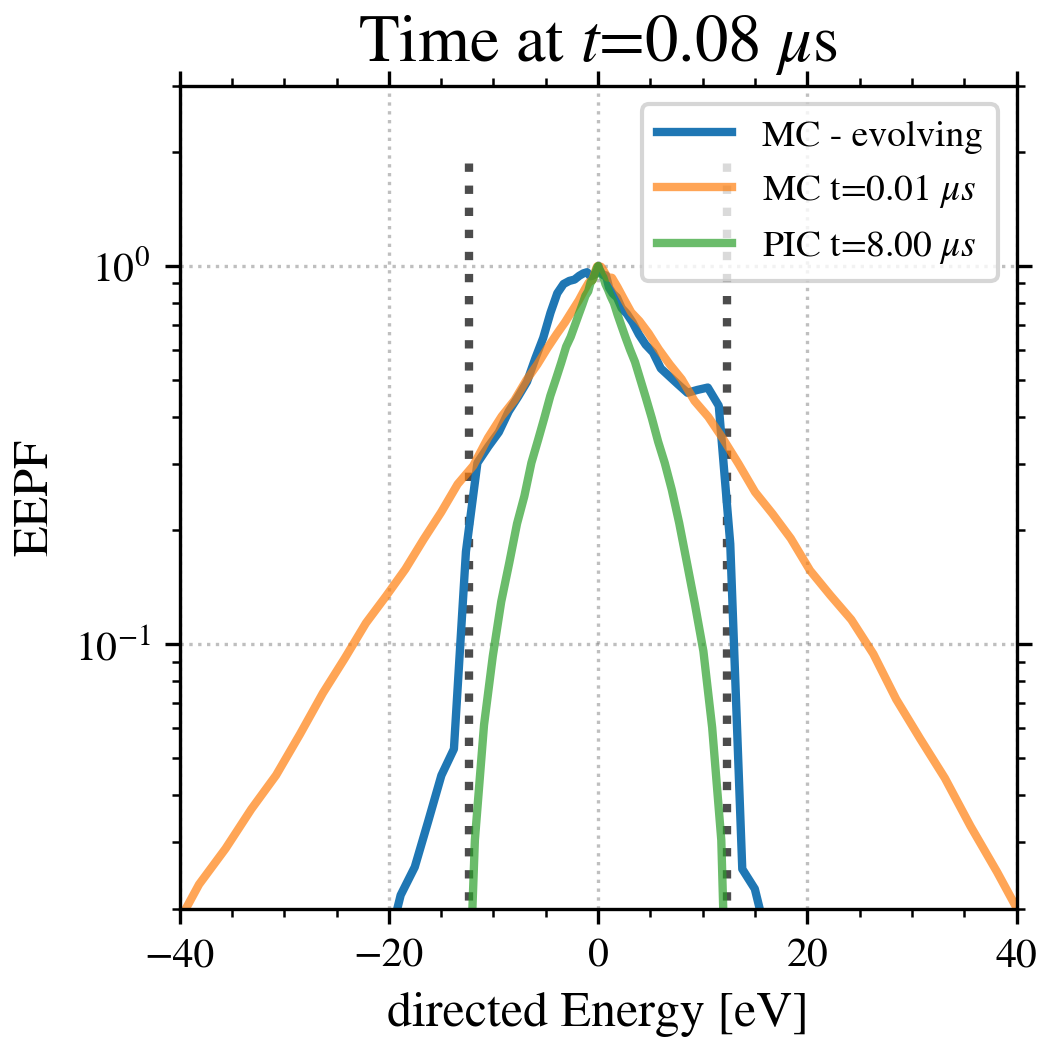
\includegraphics[width=0.4\textwidth]{MCC_EEDF/Heelo_8} \\
      \end{tabular}
      \caption{Evolution of the directed EEPF measured at $x=3\,\centi\meter$ from a wall. The positive energy is used for the electron going from the wall, while the negative energy represents the electrons moving toward the wall. The dotted line correspond to the local potential. Are overlaid (organge) the initial Maxwellian distribution and (green) the EEPF obtained at the end of the \ac{PIC} simulation. }
      \label{fig-zoom_init_Mc}
    \end{figure}

    Two phenomena can be seen in \cref{fig-zoom_init_Mc}.
    The first is the rapid decrease of the tail of the distribution function, for energies higher than the plasma potential.
    The tail for positive energy decreases faster than for negative energy, as the EEPF is measured closer to one wall than the other ($x=3\,\centi\meter$ against $L-x=7\,\centi\meter$).
    As expected, after $ T_{\rm flight}\simeq 0.07\,\micro\second$ the two tails are largely depleted, as they are one order of magnitude smaller than the Maxwellian EEPF.

    The second phenomena is the presence of waves in the velocity space that can be seen in the low energy populations.
    They are due to the plasma potential profiles.
    Indeed, the electrons are initialized with a uniform temperature, but their total energy depends on the local plasma potential. 

    \Cref{fig-zoom_Mc_later} shows the evolution of the EEDF over a longer time scale from $t=0.1$ to $2\,\micro\second$ compared to \cref{fig-zoom_init_Mc}.
    We can see the slow evolution of the low energy population from the initial, but slightly perturbed, Maxwellian distribution toward a distribution of smaller temperature.
    After $t=2\,\micro\second$, the EEPF of the Monte Carlo computation is fairly close to the \ac{PIC} EEPF.
    This is significantly longer than the estimated time scale of the elastic collisions ${T_{\rm ela}  = 0.4 \,\micro\second }$.
    \inlinenote{Why so ?? Est-ce que c'est parce que $T_{ela}$ est mal calculé ?}

    \begin{figure}[hbtp]
      \begin{tabular}{ccc}
        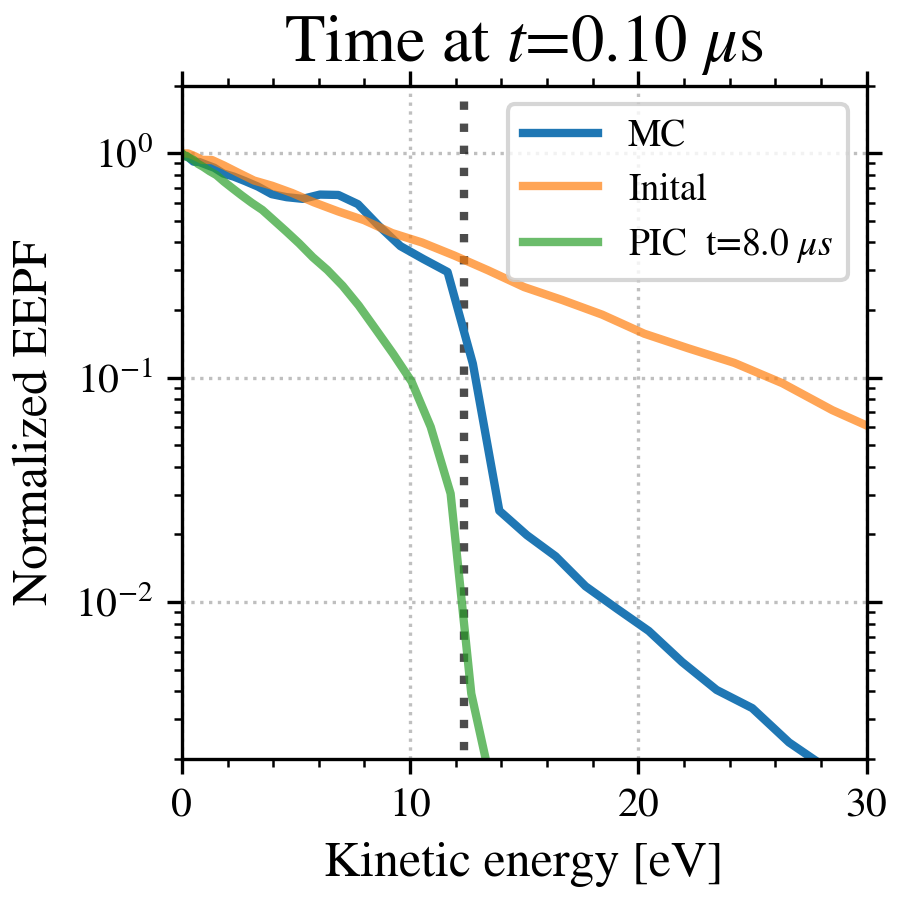
\includegraphics[width=0.3\textwidth]{MCC_EEDF/Heelo_1_10} &
        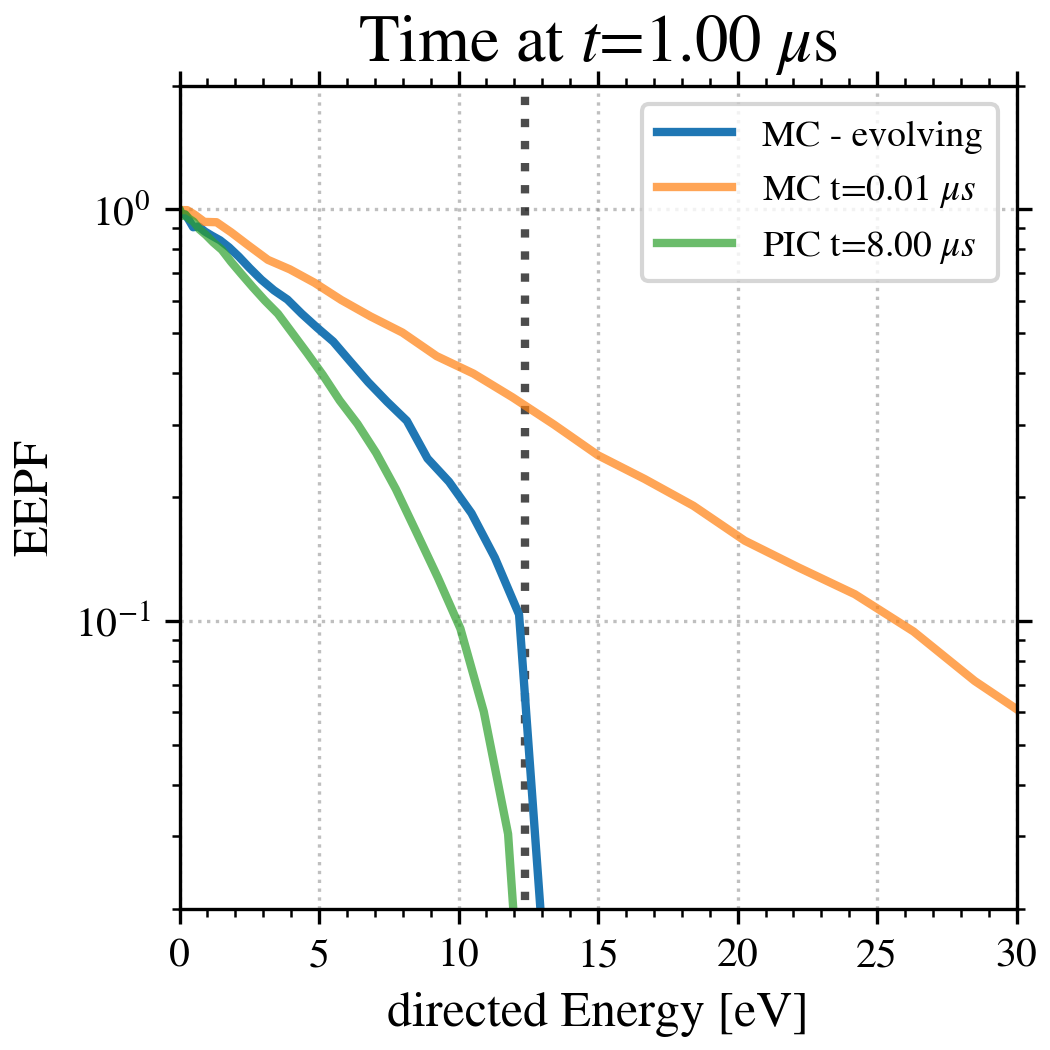
\includegraphics[width=0.3\textwidth]{MCC_EEDF/Heelo_1_100} &
        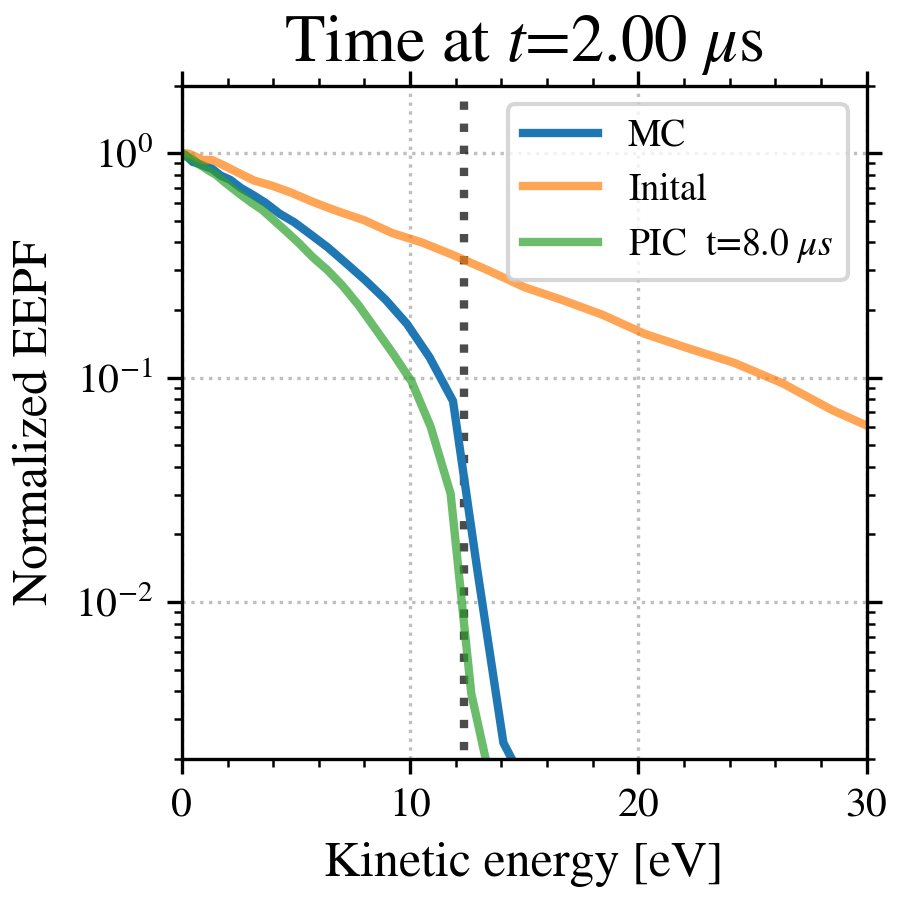
\includegraphics[width=0.3\textwidth]{MCC_EEDF/Heelo_1_200} \\
      \end{tabular}
      \caption{Evolution of the directed EEPF measured at $x=3\,\centi\meter$ from a wall. The dotted line corresponds to the local potential. Are overlaid (organge) the initial Maxwellian distribution and (green) the EEPF obtained at the end of the \ac{PIC} simulation. }
      \label{fig-zoom_Mc_later}
    \end{figure}
    \unsure{The legend can be improved here}

    \vspace{1em}
    This Monte Carlo investigation has shown that in the \ac{1D} model, the EEPF depends on the absorption at the wall but also the electron-neutral collisions.
    The final shape of the distribution is not simple, and is difficult to described and predict analytically.
    However, given the potential profile, the Monte Carlo computation reproduces the same distribution in a much shorter time compared to the \ac{PIC} simulation. 
    The obtained EEPF can then be used to determine the electron density and temperature evolution.
    This could be used to determine efficiently, and precisely, the electron polytropic coefficient.
